\documentclass[conference]{IEEEtran}

\IEEEoverridecommandlockouts
\usepackage{cite}
\usepackage{amsmath,amssymb,amsfonts}
\usepackage{graphicx}
\usepackage{textcomp}
\usepackage{xcolor}
\usepackage{optidef}
\usepackage{makecell}
\usepackage{booktabs}
\usepackage{multirow}
\usepackage{diagbox}
\usepackage{indentfirst}
\usepackage{float}
\usepackage{algorithm}
\usepackage{algpseudocode}
\usepackage{nicematrix}
\usepackage{hyperref}
\def\BibTeX{{\rm B\kern-.05em{\sc i\kern-.025em b}\kern-.08em
    T\kern-.1667em\lower.7ex\hbox{E}\kern-.125emX}}

\begin{document}

\title{Regularization techniques for a Riccati-based Interior-Point QP Solver}

\author{
    \IEEEauthorblockN{Jingtao Xiong}
    \IEEEauthorblockA{
        jingtao.xiong@email.uni-freiburg.de
    }
    \and
    \IEEEauthorblockN{Jonathan Frey}
    \and
    \IEEEauthorblockN{Katrin Baumgärtner}
    \and
    \IEEEauthorblockN{Moritz Diehl}
}
\maketitle

\begin{abstract}
This report presents regularization techniques for a Riccati-based Interior-Point Method (IPM) designed to solve Optimal Control Problem (OCP) structured indefinite Quadratic Programs (QPs).
We explore and compare Full Hessian and Reduced Hessian regularization methods, specifically focusing on Eigenvalue Modification techniques to handle indefinite QPs.
Numerical experiments demonstrate that regularizing the Reduced Hessian during Riccati recursion avoids over-regularization and improves performance compared to Full Hessian approaches.
\end{abstract}

\section{Introduction and Background}
In nonlinear optimal control, Sequential Quadratic Programming (SQP) methods are widely used to solve the underlying optimization problems\cite{verschueren2020acadosmodularopensourceframework},
where each iteration involves solving a Quadratic Program (QP) that approximates the original problem.
As a result, the efficiency and robustness of the QP solver are crucial for the overall performance of the SQP method.

Currently, Convex QP solvers are commonly employed \cite{osqp}\cite{Ferreau2014}\cite{arnstrom2022dual}. Especially for convex QPs with an Optimal Control Problem (OCP) structure,
Riccati recursion is particularly efficient due to their ability to exploit the problem's structure, achieving linear complexity in the number of stages $N$\cite{gianluca2013efficient}.
However, when the Hessian of the QP formulation is indefinite, convex QP solvers may not be able to find a descent direction,
which gives rise to the need for regularization to recover positive definiteness for the QPs.

Most existing regularization techniques can be categorized as:
\begin{itemize}
    \item \textbf{Eigenvalue Modification (EM)}: This approach modifies the Hessian by adjusting its eigenvalues to ensure positive definiteness, often by adding a small positive constant to the eigenvalues or taking their absolute values.
    \item \textbf{Cholesky Modification (CM)}: This method modifies the Cholesky factorization process to handle indefinite matrices, typically by adding a small positive value to the diagonal elements during factorization.
    \item \textbf{Levenberg-Marquardt (LM)}: This technique adds a scaled identity matrix to the Hessian, effectively shifting its eigenvalues to ensure positive definiteness.
\end{itemize}

In this report, we investigate regularization techniques based on Eigenvalue Modification and evaluate their application on the Full Hessian versus the Reduced Hessian within a Riccati-based IPM.

\section{Problem Formulation}
Consider a QP with equality $Fy=b$ and inequality constraints $Gy \le d$. By introducing slack variables $t$, we have the following formulation:

\begin{mini}
    {y, t}
    {\frac{1}{2} y^T H y + g^T y}
    {\label{eq:qp_problem}}
    {}
    \addConstraint{F y}{= b}
    \addConstraint{G y + t}{= d}
    \addConstraint{t}{\ge 0}
\end{mini}
the corresponding KKT conditions are:
    \begin{equation}
        r(y, t, \pi, \lambda) =
        \begin{bmatrix}
            H y + g + F^T \pi + G^T \lambda \\
            F y - b \\
            G y + t - d \\
            T \Lambda \mathbf{1} - \sigma \mu \mathbf{1}
        \end{bmatrix} = 0
    \end{equation}
where $T = \mathrm{diag}(t)$, $\Lambda = \mathrm{diag}(\lambda)$, $\pi$ and $\lambda$ are dual variables for equality and inequality constraints respectively,
$\sigma$ is the centering parameter and $\mu$ is the duality measure.

At each iteration $i$, we apply newton's method to solve the above KKT system, 
by defining the residuals as:
\begin{equation}
        \begin{bmatrix}
		r_{\mathrm{stat}}^i \\
		r_{\mathrm{eq}}^i \\
		r_{\mathrm{ineq}}^i \\
		r_{\mathrm{comp}}^i
		\end{bmatrix}
        =
		\begin{bmatrix}
            Hy_i + g + F^T \pi_i + G^T \lambda_i \\
            Fy_i - b \\
            Gy_i + t_i - d \\
            T_i \Lambda_i \mathbf{1} - \sigma_i \mu_i \mathbf{1}
        \end{bmatrix}
\end{equation}
we have the following linearized system:
	\begin{equation}
		\begin{bmatrix}
		H & F^T & G^T & 0\\
		F & 0 & 0 & 0 \\
		G & 0 & 0 & I \\
		0 & 0 & T_i & \Lambda_i
		\end{bmatrix}
		\begin{bmatrix}
		\Delta y \\
		\Delta \pi \\
        \Delta \lambda \\
		\Delta t
		\end{bmatrix} = -
		\begin{bmatrix}
		r_{\mathrm{stat}}^i \\
		r_{\mathrm{eq}}^i \\
		r_{\mathrm{ineq}}^i \\
		r_{\mathrm{comp}}^i
		\end{bmatrix}
	\end{equation}

By eliminating $\Delta t$ and $\Delta \lambda$ using the Schur Complement, we obtain the Reduced system:

\begin{equation}
    \begin{bmatrix}
    \tilde{H} & F^T \\
    F & 0
    \end{bmatrix}
    \begin{bmatrix}
    \Delta y \\
    \Delta \pi
    \end{bmatrix} = -
    \begin{bmatrix}
    \tilde{r}_{\mathrm{stat}}^i \\
    r_{\mathrm{eq}}^i
    \end{bmatrix}
\end{equation}
where the $\tilde{H} = H + G^T \Lambda_i T_i^{-1} G$ and $\tilde{r}_{\mathrm{stat}}^i = r_{\mathrm{stat}}^i - G^T T_i^{-1} ( \Lambda_i r_{\mathrm{ineq}}^i - r_{\mathrm{comp}}^i )$.
The $G^T \Lambda_i T_i^{-1} G$ represents the curvature contribution from inequality constraints.

For QPs with an OCP structure, by interleaving the state, control, and dual variables across $N$ stages, 
the KKT system exhibits a block-tridiagonal structure, shown as follows:
\begin{equation*}
    \begin{bNiceMatrix}[margin]
        \ddots & & & & \\
        & 0 & -I \\
        & -I & \tilde{Q}_k & \tilde{S}_k^T & A_k^T \\
        & 0 & \tilde{S}_k & \tilde{R}_k & B_k^T \\
        & 0 & A_k & B_k & 0 \\
        &  &  &  &  & \ddots
    \CodeAfter
        \SubMatrix({3-3}{4-4})
    \end{bNiceMatrix}
    \begin{bmatrix}
        \vdots \\
        \Delta \pi_k \\
        \Delta x_k \\
        \Delta u_k \\
        \Delta \pi_{k+1}\\
        \vdots
    \end{bmatrix} = -
    \begin{bmatrix}
        \vdots \\
        r_{\mathrm{eq}}^{k-1} \\
        \tilde{r}_{\mathrm{stat}, x}^k \\
        \tilde{r}_{\mathrm{stat}, u}^k \\
        r_{\mathrm{eq}}^k \\
        \vdots
    \end{bmatrix}
\end{equation*}
where the matrix $\tilde{H}_k$ decomposes into the state cost $\tilde{Q}_k$, control cost $\tilde{R}_k$, and cross-term cost $\tilde{S}_k$, alongside dynamics matrices $A_k$ and $B_k$.

This structure allows the reduced system to be solved in $\mathcal{O}(N)$ via Riccati recursion, 
consisting of a backward recursion to compute the reduced Hessian $M_k = \tilde{R}_k + B_k^T P_{k+1} B_k$ and the cost-to-go matrix $P_k$ as well as the corresponding linear term,
followed by a forward recursion to recover the search directions $\Delta u_k, \Delta x_{k+1}, \Delta t_k$ and $\Delta \lambda_k$\cite{rao1998application}\cite{frison2020hpipmhighperformancequadraticprogramming}, 
the algorithm is shown in the pseudocode \ref{alg:riccati_recursion}:

\begin{algorithm}
\caption{Riccati Recursion for Solving OCP Structure QP}
\label{alg:riccati_recursion}
\begin{algorithmic}[1]
\State\textbf{Initialize:} $P_N \gets \tilde{Q}_N$, $p_N \gets \tilde{r}_{\mathrm{stat}, x}^N$

\Statex 
\Statex\textbf{// Backward recursion}
\For{$k = N-1$ \textbf{down to} $0$}
    \State $M_k \gets \tilde{R}_k + B_k^T P_{k+1} B_k$
    \State $W_k \gets \tilde{S}_k + B_k^T P_{k+1} A_k$
    \State $K_k \gets -M_k^{-1} W_k$
    \State $k_k \gets -M_k^{-1} \left(\tilde{r}_{\mathrm{stat}, u}^k + B_k^T (P_{k+1} r_{\mathrm{eq}}^k + p_{k+1})\right)$
    \State $P_k \gets \tilde{Q}_k + A_k^T P_{k+1} A_k - W_k^T M_k^{-1} W_k$
    \State $p_k \gets \tilde{r}_{\mathrm{stat}, x}^k + A_k^T (P_{k+1} r_{\mathrm{eq}}^k + p_{k+1}) + W_k^T k_k$
\EndFor

\Statex
\Statex \textbf{// Forward recursion}
\For{$k = 0$ \textbf{to} $N-1$}
    \State $\Delta u_k \gets K_k \Delta x_k + k_k$
    \State $\Delta x_{k+1} \gets A_k \Delta x_k + B_k \Delta u_k + r_{\mathrm{eq}}^k$
    \State $\Delta t_k \gets -(G_{x}^k \Delta x_k + G_{u}^k \Delta u_k + r_{\mathrm{ineq}}^k)$
    \State $\Delta \lambda_k \gets T_k^{-1} (-r_{\mathrm{comp}}^k - \Lambda_k \Delta t_k)$
\EndFor
\end{algorithmic}
\end{algorithm}

\section{Regularization Techniques}
In indefinite QPs, the regularization can be applied to either the Full Hessian $\tilde{H}$ or the Reduced Hessian $M$ during the Riccati recursion,
the resulted regularized Reduced KKT system can be generally presented as:

\begin{equation}
    \begin{bmatrix}
     \tilde{H} + E & F^T \\
    F & 0
    \end{bmatrix}
    \begin{bmatrix}
    \Delta y \\
    \Delta \pi
    \end{bmatrix} = -
    \begin{bmatrix}
    \tilde{r}_{\mathrm{stat}}^i \\
    r_{\mathrm{eq}}^i
    \end{bmatrix}
\end{equation}
where $E$ is the adjustment matrix for ensuring positive definiteness of the original Hessian.

\subsection{Hessian-based Regularization}
To ensure the positive definiteness of the Full Hessian $H_k$ at stage $k$,
two kinds of eigenvalue decomposition are usually leveraged while maintain the sparsity of the system\cite{verschueren2017sparsity}.

Assuming the eigenvalue decomposition of hessian at stage $k$ can be written as $H_k = V_k D_k V_k^T$,
where $V_k$ is an orthogonal matrix of eigenvectors, $D_k$ is a diagonal matrix of real eigenvalues.
We have the following two variants of eigenvalue modification for regularization:
\begin{itemize}
    \item \textbf{PROJECT} (Eigenvalue Truncation):
    \begin{equation*}
        \mathrm{project}(H_k, \epsilon) := V_k \max(\epsilon I, D_k) V_k^T
    \end{equation*}
    This approach clips any negative or near-zero eigenvalues to a small positive constant $\epsilon > 0$.
    It effectively flattens directions of negative curvature with a small modification to the original Hessian.

    \item \textbf{MIRROR} (Absolute Value Modification):
    \begin{equation*}
        \mathrm{mirror}(H_k, \epsilon) := V_k \max(\epsilon I, |D_k|) V_k^T
    \end{equation*}
    This method reflects negative eigenvalues to their positive counterparts. 
    It preserves the magnitude of the curvature in all directions, which often provides better scaling,
    but may result in a large modification to the original matrix.
\end{itemize}

The primary advantage of full Hessian regularization is its robustness, as it directly ensures the positive definiteness of the full Hessian matrix,
and also it ensures the minimal Frobenius norm adjustment to the original Hessian\cite{nocedal2006numerical}.

However, full Hessian regularization, while robust, often ignores the definiteness of the reduced Hessian $M_k$, 
which can promise a feasible descent direction when positive, and thus leads to over-regularization and unnecessary computational overhead.

\subsection{Reduced-Hessian-Based Regularization}
To overcome these drawbacks, we propose an on-the-fly regularization strategy that targets the reduced Hessian 
\begin{equation*}
    M_k = R_k + B_k^T P_{k+1} B_k
\end{equation*}
directly during the backward Riccati recursion. This intervention is dynamically triggered whenever the Cholesky factorization of $M_k$ fails (i.e., when $M_k$ is detected to be non-positive definite).

Let \(\mathcal{E}(\cdot, \epsilon) \in \{\mathrm{project}(\cdot, \epsilon), \mathrm{mirror}(\cdot, \epsilon)\}\) denote the chosen eigenvalue modification operator. We introduce the following three structure-exploiting techniques:

\begin{itemize}
    \item \textbf{M\_STAGE\_EM} (Direct $M_k$ Modification): 
    The most straightforward approach applies the eigenvalue modification directly to the assembled reduced Hessian:
    \begin{equation*}
        \tilde{M}_k = \mathcal{E}(M_k, \epsilon)
    \end{equation*}

    \item \textbf{PM\_STAGE\_EM} (Cost-to-Go Modification): 
    Negative curvature often propagates backward through time via the cost-to-go matrix $P_{k+1}$. 
    In this variant, we first regularize $P_{k+1}$ before assembling $M_k$, and then apply a secondary safeguard to the resulting $M_k$:
    \begin{equation*}
        \begin{aligned}
            \tilde{P}_{k+1} &= \mathcal{E}(P_{k+1}, \epsilon) \\
            \hat{M}_k &= R_k + B_k^T \tilde{P}_{k+1} B_k \\
            \tilde{M}_k &= \mathcal{E}(\hat{M}_k, \epsilon)
        \end{aligned}
    \end{equation*}

    \item \textbf{RP\_STAGE\_EM} (Stage Cost and Cost-to-Go Modification): 
    This method implicitly regularizes the reduced hessian, by regularizing both the control penalty matrix $R_k$ and the cost-to-go matrix $P_{k+1}$ prior to forming the reduced Hessian:
    \begin{equation*}
        \begin{aligned}
            \tilde{R}_k &= \mathcal{E}(R_k, \epsilon) \\
            \tilde{P}_{k+1} &= \mathcal{E}(P_{k+1}, \epsilon) \\
            \tilde{M}_k &= \tilde{R}_k + B_k^T \tilde{P}_{k+1} B_k
        \end{aligned}
    \end{equation*}
\end{itemize}

All three of these reduced Hessian regularization methods can be implemented seamlessly using either the PROJECT or MIRROR variants discussed previously.

\section{Numerical experiments}

\subsection{Experiments setup}
For our numerical experiments, we focus on solving unconstrained optimal control problems as follows:

With the stage cost $l(x_k, u_k)$ at each time step as:
\begin{equation}
    \begin{aligned}
        l(x_k, u_k) =& \frac{1}{2} \begin{bmatrix} x_k \\ u_k \end{bmatrix}^T 
        \begin{bmatrix} Q_k & S_k^T \\ S_k & R_k \end{bmatrix} 
        \begin{bmatrix} x_k \\ u_k \end{bmatrix} \\
        &+ \begin{bmatrix} q_k \\ r_k \end{bmatrix}^T 
        \begin{bmatrix} x_k \\ u_k \end{bmatrix},
    \end{aligned}
\end{equation}
and the terminal cost $E(x_N)$ as:
\begin{equation}
    E(x_N) = \frac{1}{2} x_N^T Q_N x_N + q_N^T x_N.
\end{equation}

The QP formulation is given by:
\begin{mini*}[short] 
    {x, u} 
    { \sum_{k=0}^{N-1} l(x_k, u_k) + E(x_N) } 
    {}{} 
    \addConstraint{x_0}{= \bar{x}_0}{} 
    \addConstraint{x_{k+1}}{= A_k x_k + B_k u_k,}{\quad k = 0, \dots, N-1} 
    \addConstraint{\underline{u}}{\le u_k \le \overline{u},}{\quad k = 0, \dots, N-1} 
\end{mini*}

For testing benchmark, we designed 30 simple indefinite QP problems, including:
\begin{itemize}
    \item 2 designed cases with H indefinite M Positive
    \item 4 designed cases with H indefinite M Indefinite R Indefinite P Positive
    \item 4 designed cases with H indefinite M Indefinite R Positive P Indefinite
    \item 3 designed cases with H indefinite M Indefinite R Indefinite P Indefinite
    \item 2 indefinite Pendulum QP cases with $\mathrm{N}=50,100$, $\mathrm{nx}=4, \mathrm{nu}=1$
\end{itemize}

For each designed case, the dimensions of state and control are set to $\mathrm{nx}=3, \mathrm{nu}=2$ for simplicity,
and we give 2 different initial states, i.e. $x_0 = [5.0, 5.0, 5.0], [3.0, 3.0, 3.0]$ for designed cases, $x_0 = [0.0, \pi, 0.0, 0.0], [0.0, \frac{\pi}{3}, 0.0, 0.0] $ for pendulum cases, 
which leads to a total of 30 QP problems.

We implemented the above regularization techniques in a prototype Riccati-based IPM solver with Mehrotra predictor-corrector method \cite{Mehrotra1992implementation} in python, which is available on \url{https://github.com/Pandatheon/Primal-dual_IPM}.
As for parameters regarding iteration, we set \(\epsilon = 1\mathrm{e}-4\), with a convergence tolerance of \(1\mathrm{e}-8\) (infinity norm residuals) and a maximum of 300 iterations.

\subsection{Overall Performance}
To evaluate the performance of each method,
we compare the solved problems and iteration counts across all 30 indefinite $M$ cases, as shown in the performance profiles below:
\begin{figure}[H]
    \centering
    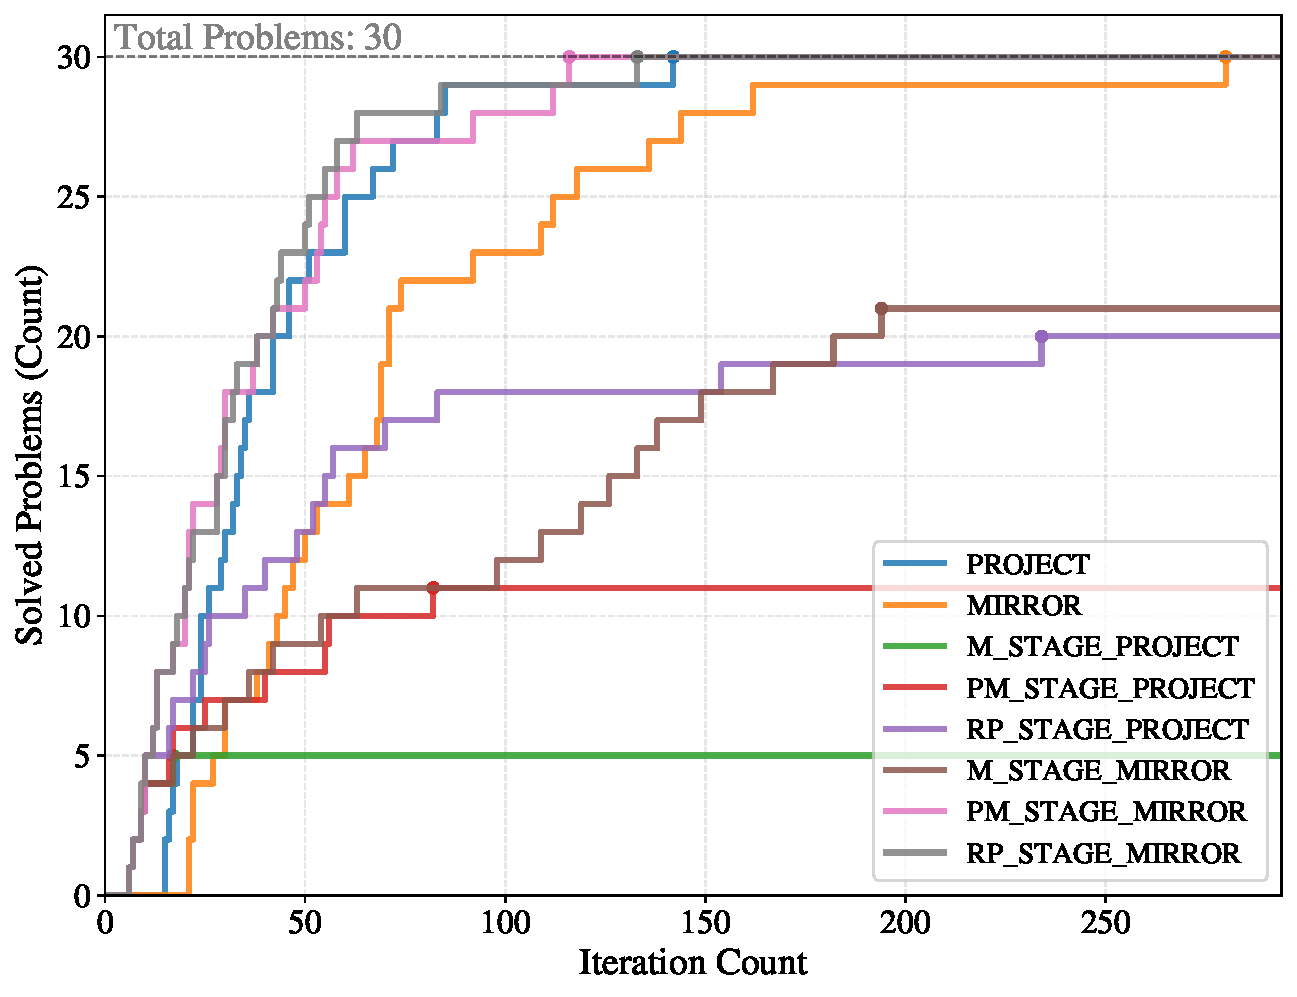
\includegraphics[width=1.0\linewidth]{figures/iteration_performance_profile.pdf}
    \caption{Performance profile comparing regularization techniques on indefinite $M$ cases.
    Only four methods PROJECT, MIRROR, RP\_STAGE\_EM and PM\_STAGE\_EM successfully solved all the 30 cases, 
    with M\_STAGE\_PROJECT as worst-performing method and both RP\_STAGE\_MIRROR, PM\_STAGE\_MIRROR as best-performing method.}
    \label{fig:performance}
\end{figure}

As shown in the figure \ref{fig:performance}, among all the regularization methods, only four methods successfully solved all the 30 cases,
which are two full Hessian regularization methods (PROJECT and MIRROR) and two reduced Hessian regularization methods (RP\_STAGE\_MIRROR and PM\_STAGE\_MIRROR).
And the two Reduced Hessian regularization methods outperform the full Hessian regularization methods in terms of iteration counts with similar performance.

Interestingly, for the full Hessian regularization methods, the PROJECT method performs better than the MIRROR method,
while for the reduced Hessian regularization methods, the MIRROR method performs better than the PROJECT method,
which indicates that the choice of regularization method can have different impacts on the performance depending on whether it is applied to the full Hessian or the reduced Hessian.

Furthermore, the regularization counts happening during the iteration are also taken into account, which is closely related to the computational overhead of the regularization techniques.
\begin{figure}[H]
    \centering
    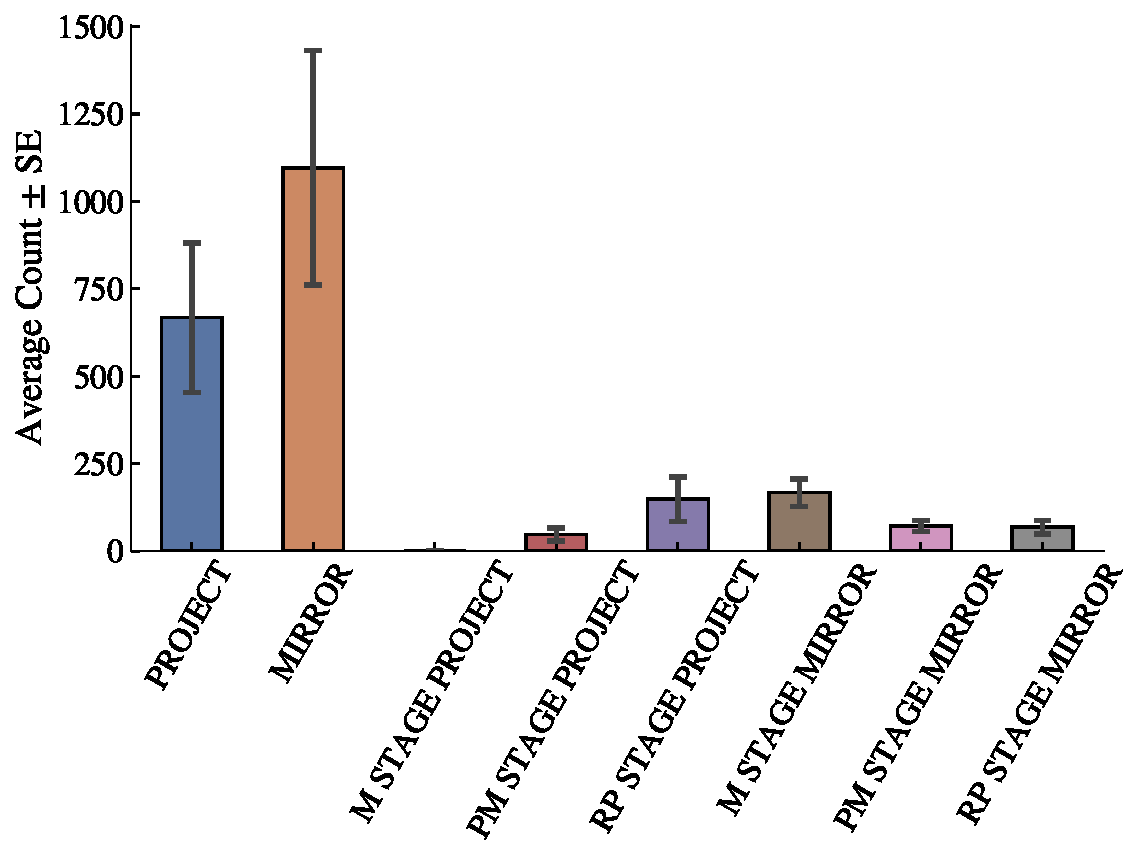
\includegraphics[width=1.0\linewidth]{figures/regularization_avg_se.pdf}
    \caption{Average regularization counts across iterations for different regularization techniques, where the error bars indicate the standard error of the mean.}
    \label{fig:reg_counts}
\end{figure}
As shown in the figure \ref{fig:reg_counts},
the reduced Hessian regularization methods generally show a significant decrease in regularization times compared to the full Hessian regularization methods,
due to the fact that the regularization, i.e. the eigenvalue decomposition, is only performed when the reduced Hessian $M$ is detected to be indefinite, 
which implies a much lower computational overhead for the reduced Hessian regularization methods.

\subsection{Case analysis}

\subsubsection{M Positive Cases}
When $M$ is positive definite, the solution is trivial for recursion-based methods to obtain a descent direction, 
and thus the solution can be obtained without any regularization,
but for the full Hessian regularization methods (PROJECT and MIRROR), the regularization is still applied to the full Hessian, 
which leads to over-regularization and thus more iterations to converge, as shown in the table\ref{tab:positive_count},
\begin{table}[H]
        \centering
        \caption{Numerical Comparison of Regularization Techniques with $x_0 = [5.0, 5.0, 5.0]$}
        \setlength{\tabcolsep}{3pt}
        \begin{tabular}{c ccc ccc}
            \toprule
            % Using multirow to span the header height
            \multirow{2}{*}{\diagbox[width=6.5em, height=2.8em]{\textbf{Reg.}}{\textbf{Problem}}} &
            \multicolumn{3}{c}{M\_pos-R\_inde-P\_pos} & \multicolumn{3}{c}{M\_pos-R\_pos-P\_inde}\\
            % 3. \cmidrule(lr) creates gaps between groups, improving scannability
            \cmidrule(lr){2-4} \cmidrule(lr){5-7}
            & Iter. & Res. & Stat. & Iter. & Res. & Stat. \\
            \midrule
            NO\_REG.    	& 7 & 3.11e-11 & 0 	    & 17 & 1.57e-10 & 0 \\
            PROJECT     	& 51 & 1.93e-16 & 0 	& 22 & 3.71e-15 & 0 \\
            MIRROR      	& 92 & 1.93e-16 & 0 	& 30 & 3.71e-15 & 0 \\
            M\_STAGE\_EM  	& 7 & 3.11e-11 & 0 	    & 17 & 1.57e-10 & 0 \\
            PM\_STAGE\_EM  & 7 & 3.11e-11 & 0 	    & 17 & 1.57e-10 & 0 \\
            RP\_STAGE\_EM  & 7 & 3.11e-11 & 0 	    & 17 & 1.57e-10 & 0 \\
            \bottomrule
        \end{tabular}
        \label{tab:positive_count}
    \end{table}

\subsubsection{M Indefinite Cases}
When \(M\) is indefinite, we focus on the reduced Hessian regularization and care about following two metrics for the reduced Hessian \(M\) and the cost-to-go matrix \(P\),
assuming the regularization is applied at iteration $i$ for stage $k$ to a QP problem:
\begin{itemize}
    \item \textbf{Maximal reduction in condition number}: A high condition number indicates a matrix is close to being singular, 
    regularization techniques should maintain or reduce the condition number to ensure numerical stability and convergence of the solver. This is calculated as:
    \begin{equation*}
        \Delta\kappa = \min\{\mathrm{cond}(M^{k,i}_{\mathrm{regularized}}) - \mathrm{cond}(M^{k,i}_{\mathrm{original}})\}
    \end{equation*}
    \item \textbf{Maximal adjustment to the eigenvalues}: This metric quantifies the magnitude of the modification applied to the original Hessian. 
    A smaller adjustment indicates less deviation from the original problem, which can help preserve the problem's structure and lead to better convergence properties.
    This is calculated as:
    \begin{equation*}
        \Delta D = \max\{D^{k,i}_{\mathrm{regularized}} - D^{k,i}_{\mathrm{original}}\}
    \end{equation*}
\end{itemize}

\begin{figure}[H]
    \centering
    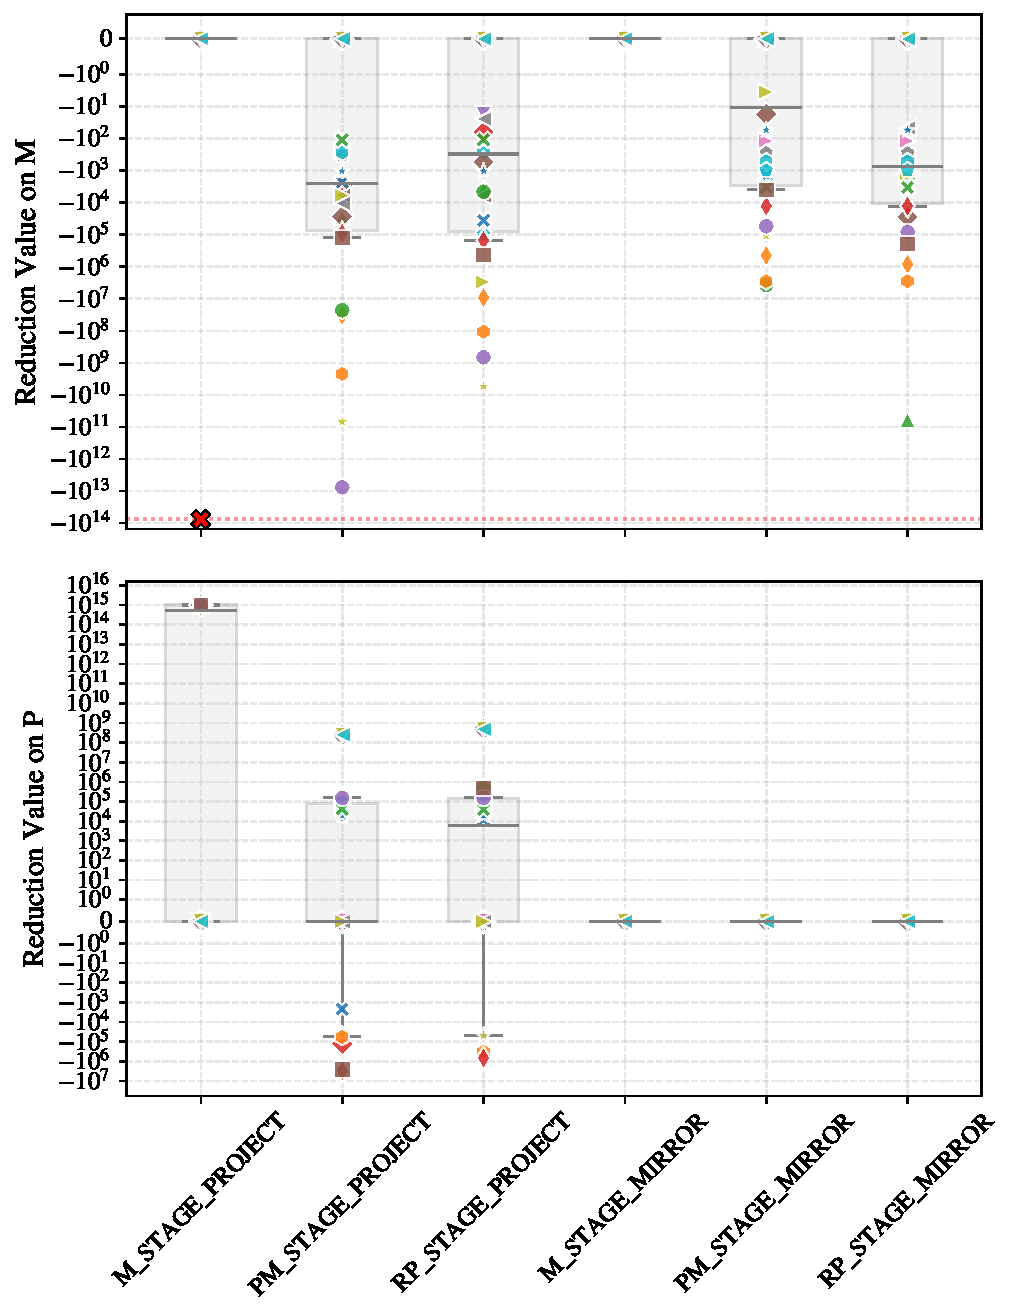
\includegraphics[width=1.0\linewidth]{figures/reduction_vertical.pdf}
    \caption{Maximal Condition number reduction of $M$ and $P$ across iterations for different regularization techniques, 
    where the negative values indicate the reduction in condition number after regularization, and the positive values indicate the increase in condition number after regularization.
    M\_STAGE\_PROJECT fail to obtain trustworthy results due to numerical issues}
    \label{fig:reduction}
\end{figure}

In figure \ref{fig:reduction}, we can see that the condition number of $M$ is generally reduced after applying regularization, 
but for the condition number of $P$,  PROJECT-based methods tend to increase the condition number of $P$ while MIRROR-based methods will maintain the original condition number of $P$.
This is because the PROJECT method clips negative eigenvalues to a small positive constant, 
which can lead to a significant increase in the condition number if the original eigenvalues were not close to zero, 
while the MIRROR method reflects negative eigenvalues to their positive counterparts, which can help maintain a more balanced spectrum of original problems.

Besides, this also provide possible explanation why the MIRROR-based methods generally outperform the PROJECT-based methods in reduced Hessian regularization, 
as a lower condition number typically leads to better numerical stability and faster convergence of the solver.

\begin{figure}[H]
    \centering
    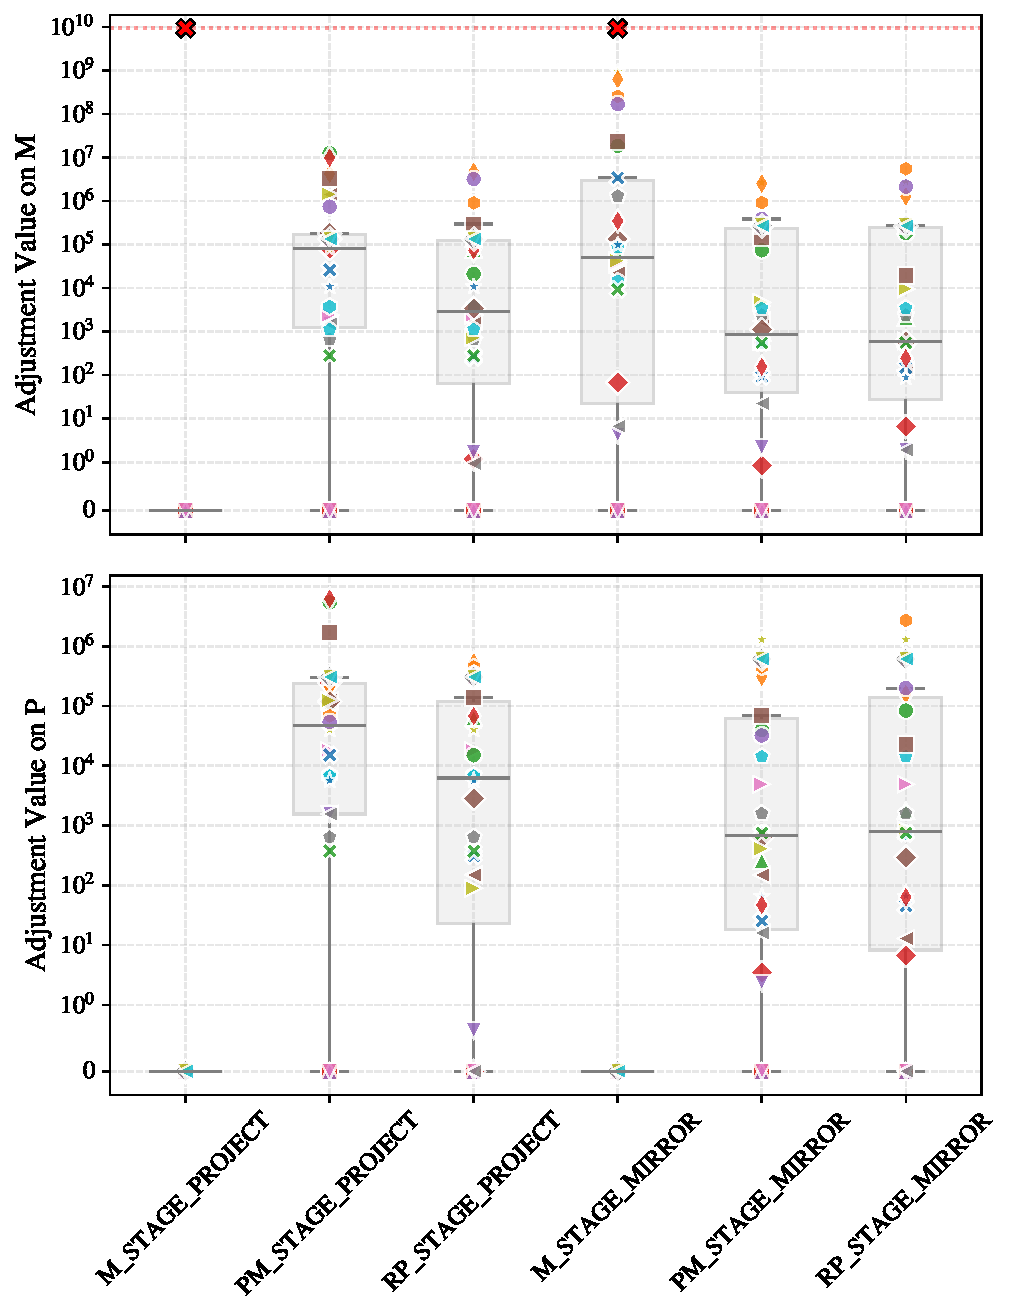
\includegraphics[width=1.0\linewidth]{figures/adjustment_vertical.pdf}
    \caption{Maximal adjustment to the eigenvalues of $M$ and $P$ across iterations for different regularization techniques.
    M\_STAGE\_PROJECT fails to obtain trustworthy results due to numerical issues}
    \label{fig:adjustment}
\end{figure}

As shown in the figure \ref{fig:adjustment},
the PM\_STAGE\_MIRROR method and the RP\_STAGE\_MIRROR generally shows the least modification to the eigenvalues of both $M$ and $P$.
This indicates that these two methods can preserve the original problem structure better than other methods, and thus lead to better convergence properties, 
consistent with the observation in the performance profiles.

\section{Conclusion}
Our numerical experiments highlight several key findings regarding regularization in Riccati-based IPM solvers for indefinite QPs with OCP structure:
\begin{itemize}
    \item \textbf{Full vs. Reduced Hessian}: Full Hessian regularization can lead to over-regularization if $M$ is already positive definite. 
    Reduced Hessian regularization avoids this by leveraging the recursion structure.
    \item \textbf{Regularization on P}: Applying regularization to $P$ within the Reduced Hessian framework generally provides significant benefits.
    \item \textbf{PROJECT vs. MIRROR}: While PROJECT typically performs better for regularizing the full Hessian, 
    MIRROR proves superior for Reduced Hessian regularization due to better control over the condition number.
\end{itemize}

% \appendix
% \section*{Additional Numerical Results: cost values}

\bibliographystyle{IEEEtran}
\bibliography{references}

\end{document}